%%%%%%%%%%%%%%%%%%%%%%%%%%%%%%%%%%%%%%%%%
% Beamer Presentation
% LaTeX Template
% Version 1.0 (10/11/12)
%
% This template has been downloaded from:
% http://www.LaTeXTemplates.com
%
% License:
% CC BY-NC-SA 3.0 (http://creativecommons.org/licenses/by-nc-sa/3.0/)
%
%%%%%%%%%%%%%%%%%%%%%%%%%%%%%%%%%%%%%%%%%

%----------------------------------------------------------------------------------------
%	PACKAGES AND THEMES
%----------------------------------------------------------------------------------------

\documentclass{beamer}

\mode<presentation> {

% The Beamer class comes with a number of default slide themes
% which change the colors and layouts of slides. Below this is a list
% of all the themes, uncomment each in turn to see what they look like.

%\usetheme{default}
%\usetheme{AnnArbor}
%\usetheme{Antibes}
%\usetheme{Bergen}
%\usetheme{Berkeley}
%\usetheme{Berlin}
%\usetheme{Boadilla}
%\usetheme{CambridgeUS}
%\usetheme{Copenhagen}
%\usetheme{Darmstadt}
%\usetheme{Dresden}
%\usetheme{Frankfurt}
%\usetheme{Goettingen}
%\usetheme{Hannover}
%\usetheme{Ilmenau}
%\usetheme{JuanLesPins}
%\usetheme{Luebeck}
\usetheme{Madrid}
%\usetheme{Malmoe}
%\usetheme{Marburg}
%\usetheme{Montpellier}
%\usetheme{PaloAlto}
%\usetheme{Pittsburgh}
%\usetheme{Rochester}
%\usetheme{Singapore}
%\usetheme{Szeged}
%\usetheme{Warsaw}

% As well as themes, the Beamer class has a number of color themes
% for any slide theme. Uncomment each of these in turn to see how it
% changes the colors of your current slide theme.

%\usecolortheme{albatross}
%\usecolortheme{beaver}
%\usecolortheme{beetle}
%\usecolortheme{crane}
%\usecolortheme{dolphin}
%\usecolortheme{dove}
%\usecolortheme{fly}
%\usecolortheme{lily}
%\usecolortheme{orchid}
%\usecolortheme{rose}
%\usecolortheme{seagull}
%\usecolortheme{seahorse}
%\usecolortheme{whale}
%\usecolortheme{wolverine}

%\setbeamertemplate{footline} % To remove the footer line in all slides uncomment this line
%\setbeamertemplate{footline}[page number] % To replace the footer line in all slides with a simple slide count uncomment this line

%\setbeamertemplate{navigation symbols}{} % To remove the navigation symbols from the bottom of all slides uncomment this line
}

\usepackage{graphicx} % Allows including images
\usepackage{booktabs} % Allows the use of \toprule, \midrule and \bottomrule in tables

%----------------------------------------------------------------------------------------
%	TITLE PAGE
%----------------------------------------------------------------------------------------

\title[Interactive 3D Human Heart Visualization]{Interactive 3D Human Heart Visualization} % The short title appears at the bottom of every slide, the full title is only on the title page

\author{C. Wurditsch \& S. Reisinger} % Your name
\institute[VC+HCT’s] % Your institution as it will appear on the bottom of every slide, may be shorthand to save space
{
TU Wien \\ % Your institution for the title page
\medskip
\textit{} % Your email address
}
\date{\today} % Date, can be changed to a custom date

\begin{document}

\begin{frame}
\titlepage % Print the title page as the first slide
\end{frame}

\begin{frame}
\frametitle{Overview} % Table of contents slide, comment this block out to remove it
\tableofcontents % Throughout your presentation, if you choose to use \section{} and \subsection{} commands, these will automatically be printed on this slide as an overview of your presentation
\end{frame}

%----------------------------------------------------------------------------------------
%	PRESENTATION SLIDES
%----------------------------------------------------------------------------------------

\section{Introduction} 

\begin{frame}
\frametitle{Introduction}
\begin{figure}[h]
  \centering
  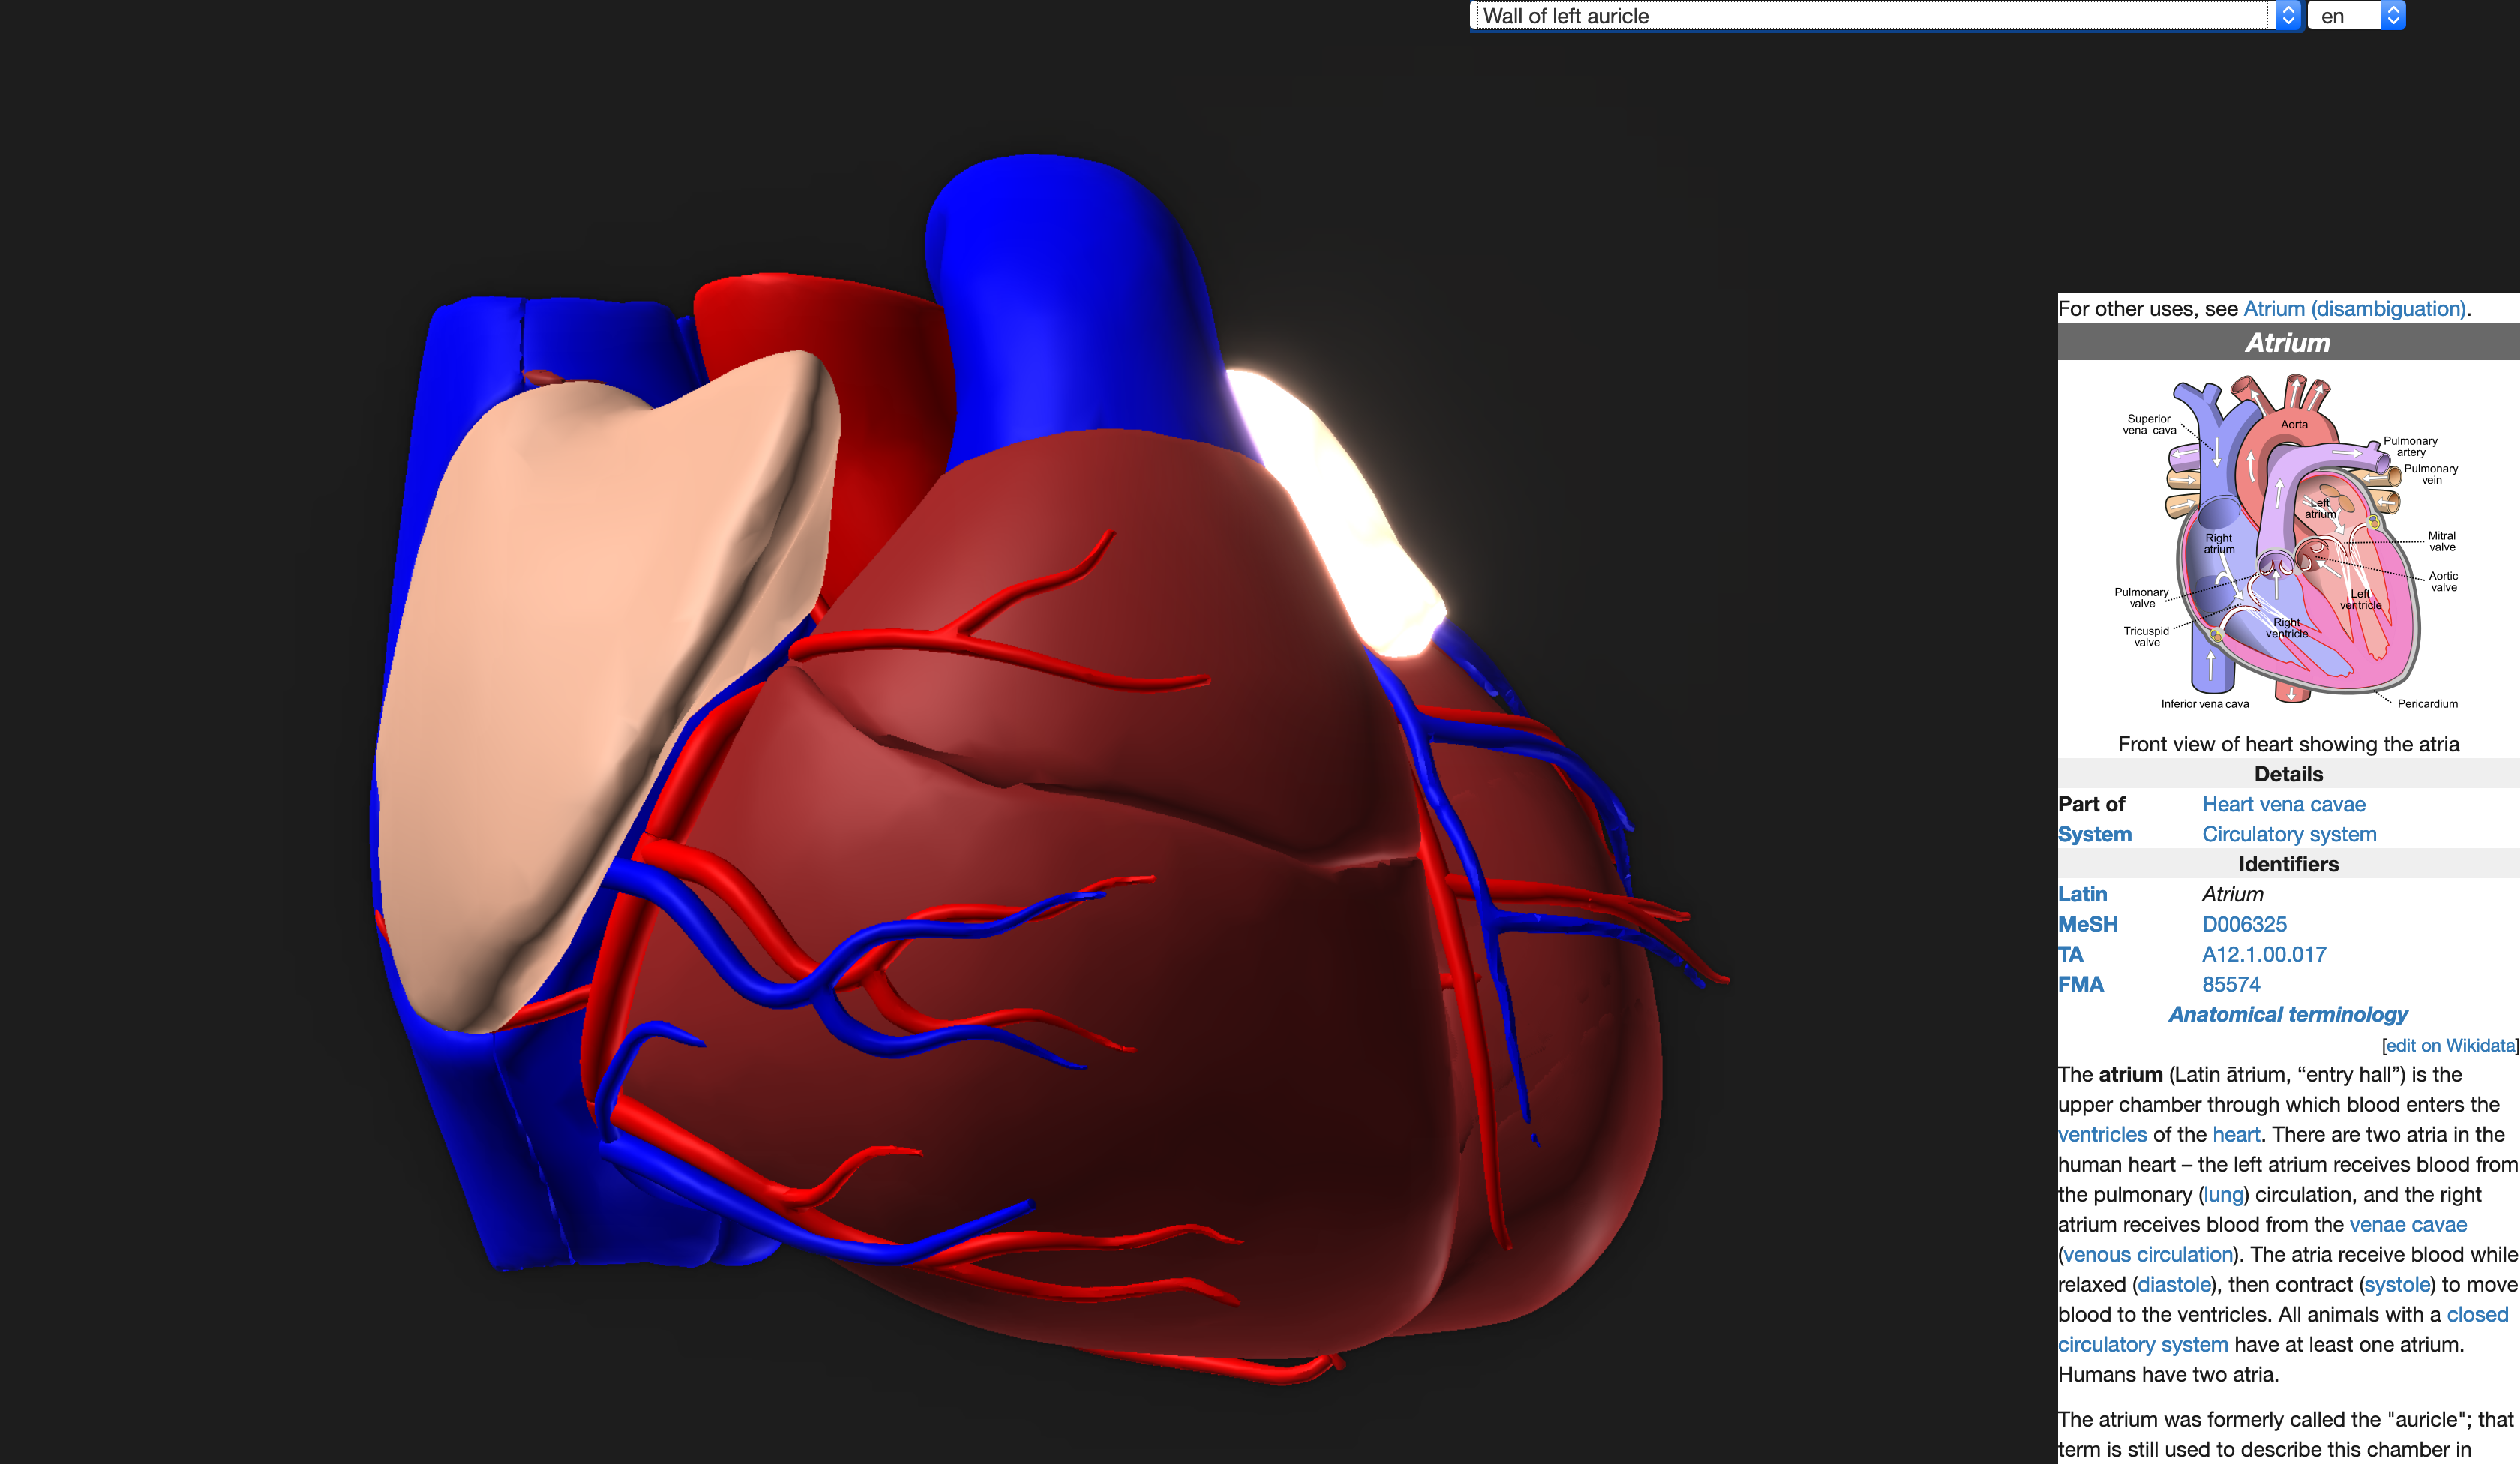
\includegraphics[width=0.9\linewidth]{../../screenshots/images/Wall_Of_Left_Auricle_highlighted.png}
\end{figure}
\end{frame}

\begin{frame}
\frametitle{Introduction - Motivation}
\begin{itemize}
    \item Visualizations of cardiovascular structures play an important role in diagnosis and treatment
    \item Cardiovascular visualizations can also be helpful for educational purposes to help learning and understanding anatomy
    \item Visualizations maybe superior to 2D images, especially if they are interactive
\end{itemize}
\end{frame}

\begin{frame}
\frametitle{Introduction - Key Points}
\begin{itemize}
    \item Interactive 3D visualization for learning the anatomy of the human heart
    \item Surface rendering of a mesh-model of anatomical structures of the human heart
    \item Based on framework java-script framework three.js, runs in nearly any recent version of a modern web browser
\end{itemize}
\end{frame}

\section{Related Work} 
\begin{frame}
\frametitle{Related work}
\begin{itemize}
\item We identified quite a few papers about assessment of anatomy learning benefits utilizing 3D visualizations compared to traditional methods (e. g. Atlases)
\item Several systematic reviews exist
\item Results differ, but most papers and reports show that anatomy learning with 3D models \& visualizations is beneficial compared to traditional learning approaches (e.g. \cite{p3} \cite{p4} )
\end{itemize}
\end{frame}

\section{Data} 
\begin{frame}
\frametitle{Data}
\begin{itemize}
\item 3D Models of the structures of the human heart provided by BodyParts3D \cite{p1}


\item Self aggregated list of Wikipedia Articles in English and German

\begin{figure}[h]
  \centering
  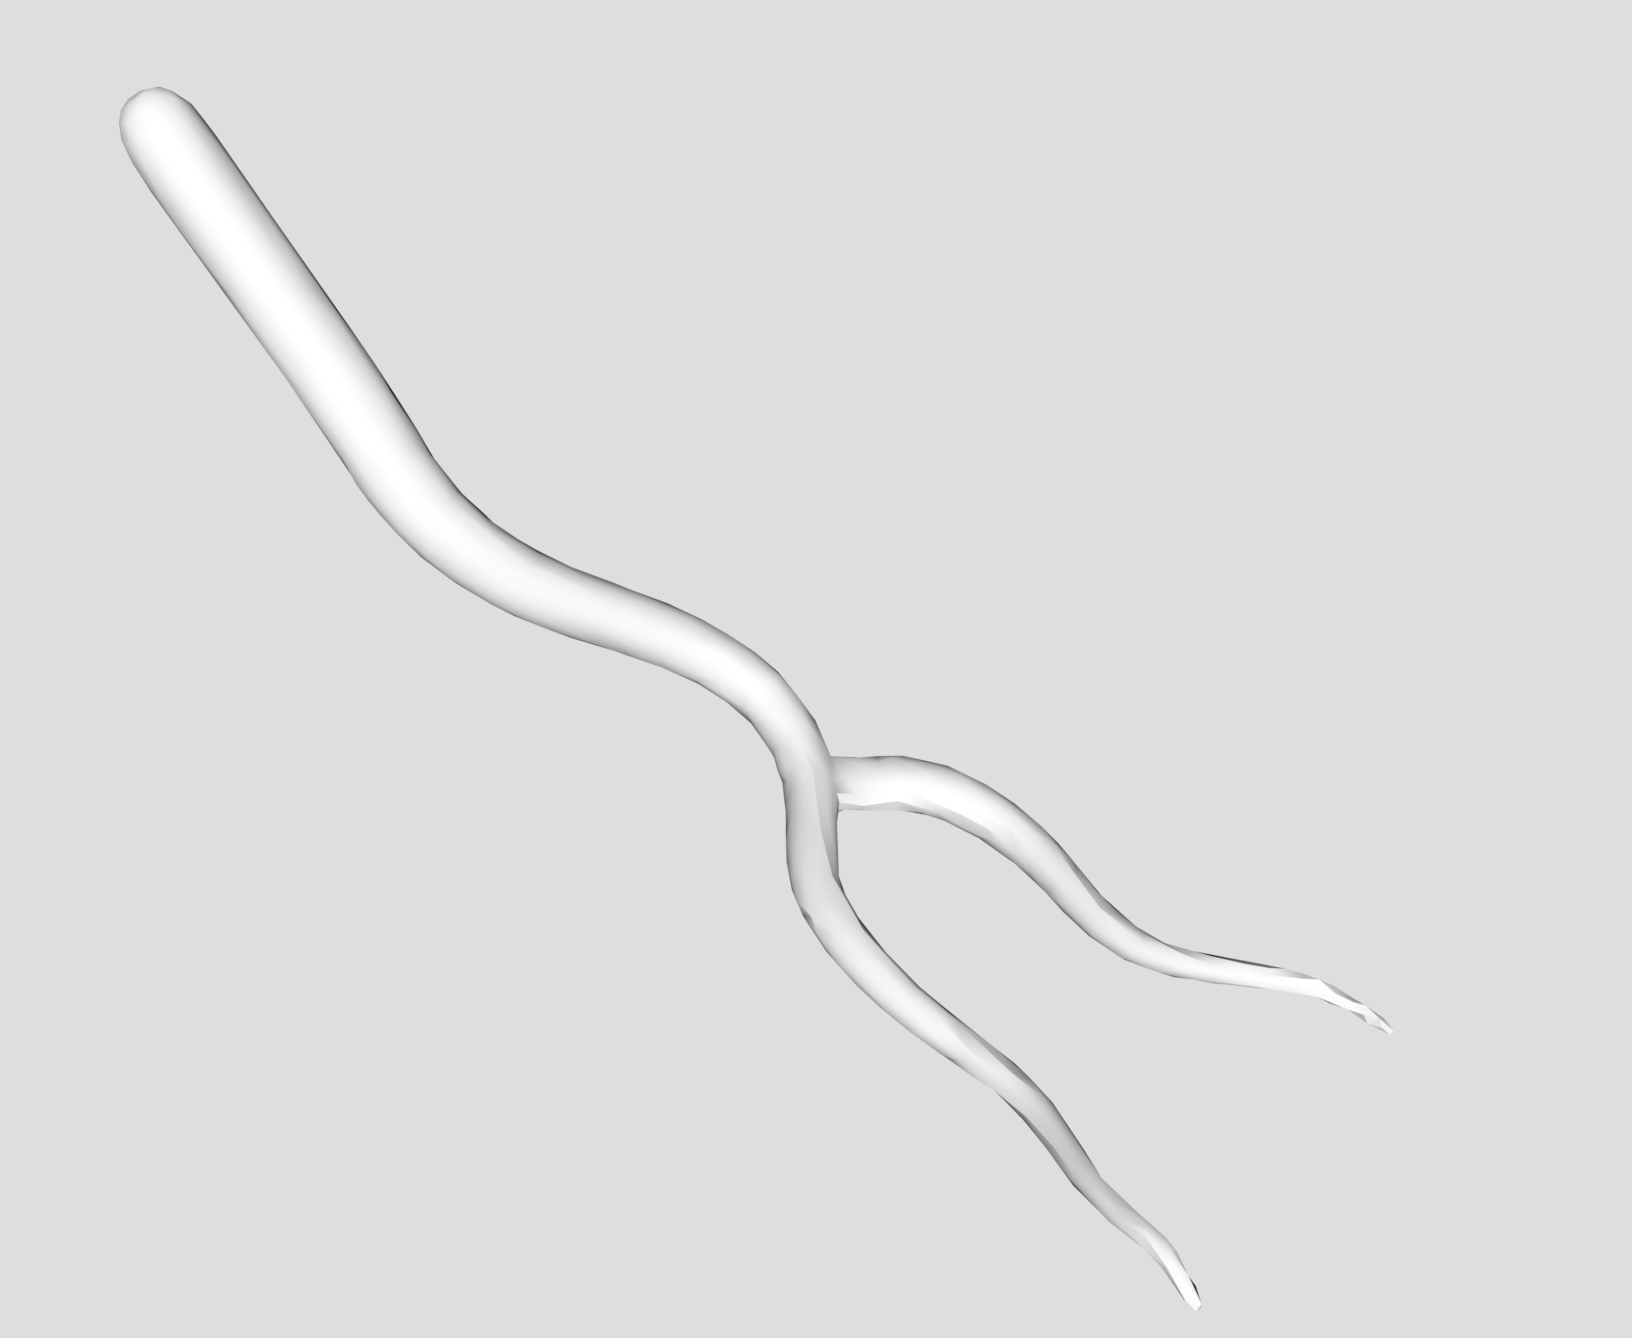
\includegraphics[width=0.4\linewidth]{../../screenshots/images/anterior_cardiac_vein.png}
  \caption{This shows the mesh model from BodyParts3D of the anterior cardiac vein.}
\end{figure}
\end{itemize}
  

\end{frame}

\begin{frame}
\frametitle{Data - Data set errors}
\begin{figure}[h]
  \begin{minipage}[b]{0.5\linewidth}
    \centering
    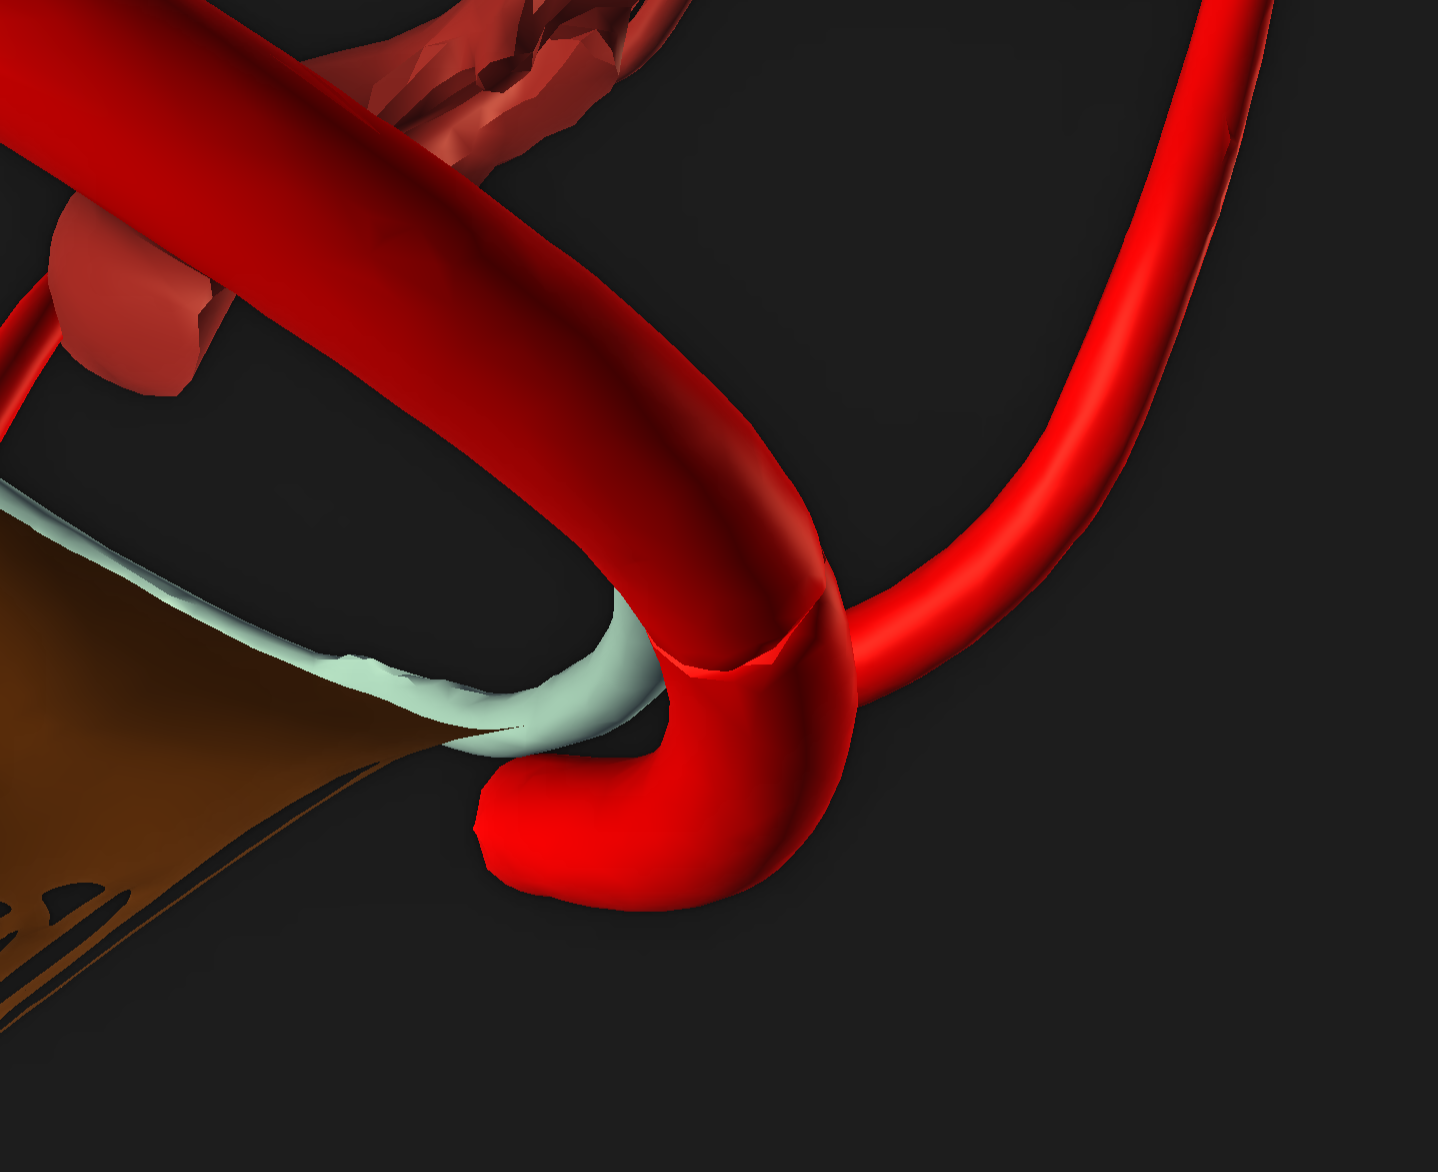
\includegraphics[width=.3\linewidth]{../../screenshots/images/error1.png} 
    \caption{Two parts of one blood vessel do not fit perfectly together}
  \end{minipage}%%
  \begin{minipage}[b]{0.5\linewidth}
    \centering
    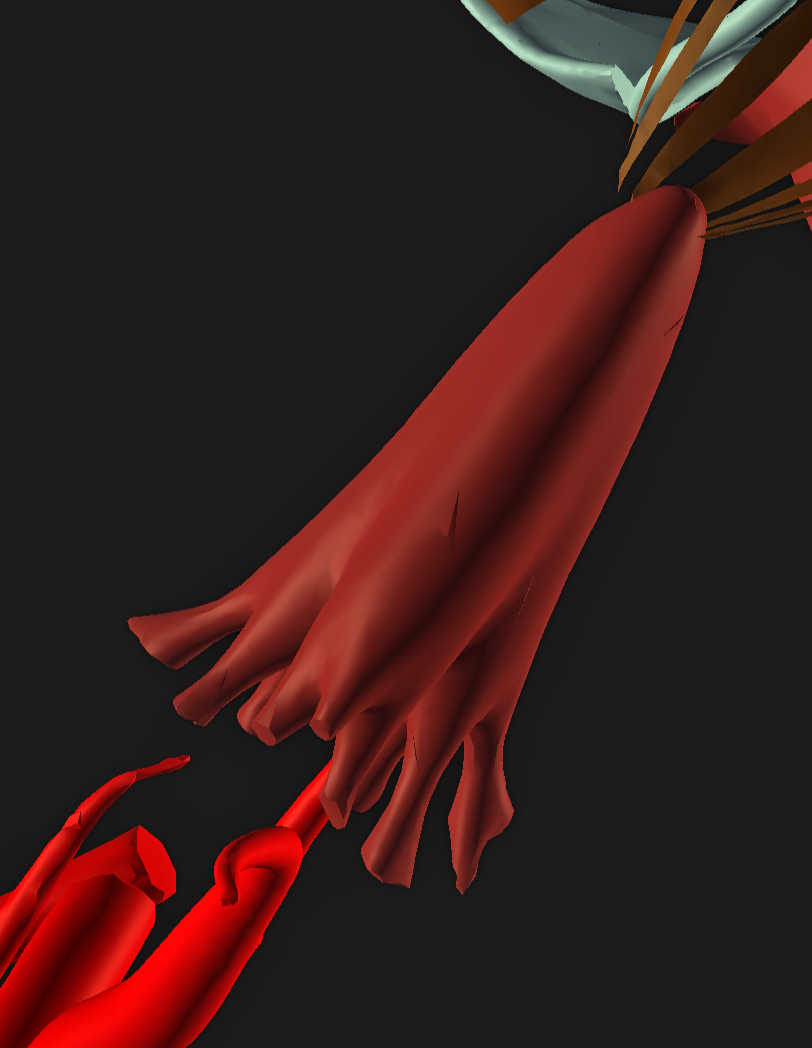
\includegraphics[width=.3\linewidth]{../../screenshots/images/error2.png} 
    \caption{Surface is not smooth}
  \end{minipage} 
  \begin{minipage}[b]{0.5\linewidth}
    \centering
    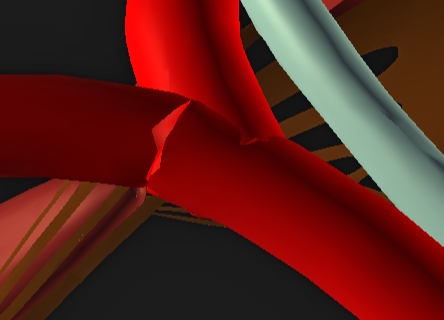
\includegraphics[width=.3\linewidth]{../../screenshots/images/error3.png} 
    \caption{Two parts of one blood vessel do not fit perfectly together}
  \end{minipage}%% 
  \begin{minipage}[b]{0.5\linewidth}
    \centering
    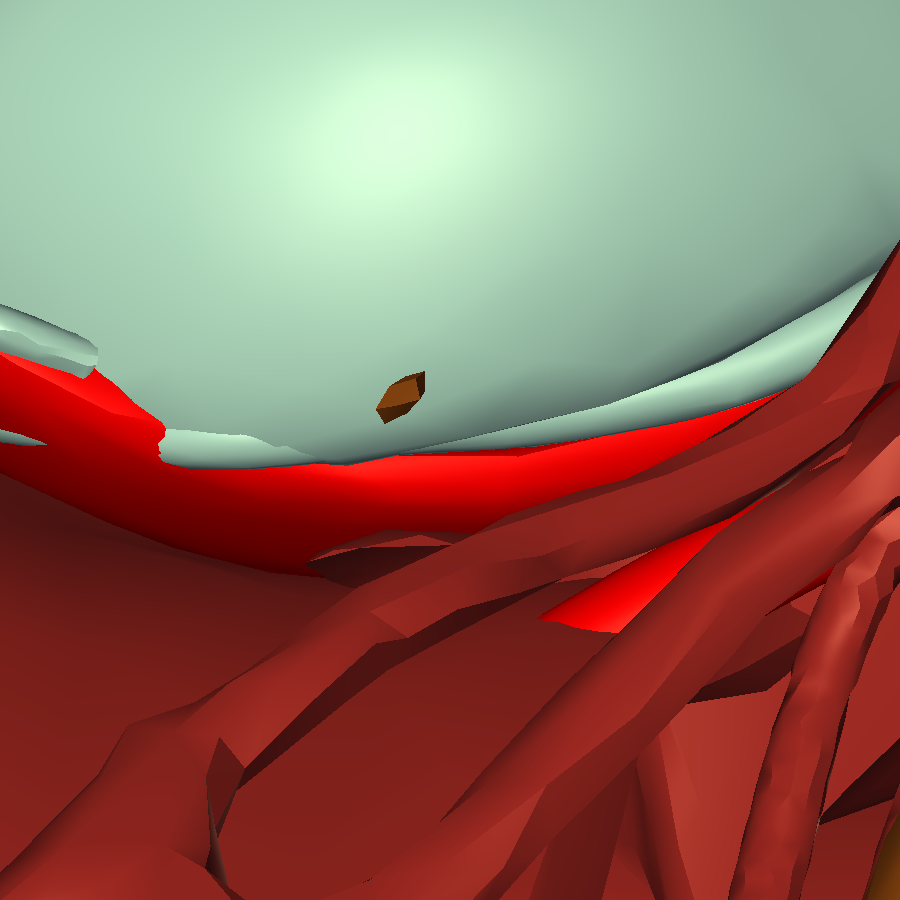
\includegraphics[width=.3\linewidth]{../../screenshots/images/error4.png} 
    \caption{There is a small object that does not belong there.}
  \end{minipage}
\caption{Artifacts of the data}
\end{figure}

\end{frame}

\section{Implementation} 

\begin{frame}
\frametitle{Implementation - Object Loading}
\begin{enumerate}
\item Loop over .obj files
\item Three.js: JLoader2Parallel for mesh loading
\item Material in the correct color created and added to the mesh. 
\item Shifted to the center of the coordinate system
\end{enumerate}
\end{frame}


\begin{frame}
\frametitle{Implementation - Rendering}
\begin{figure}[h]
  \centering
  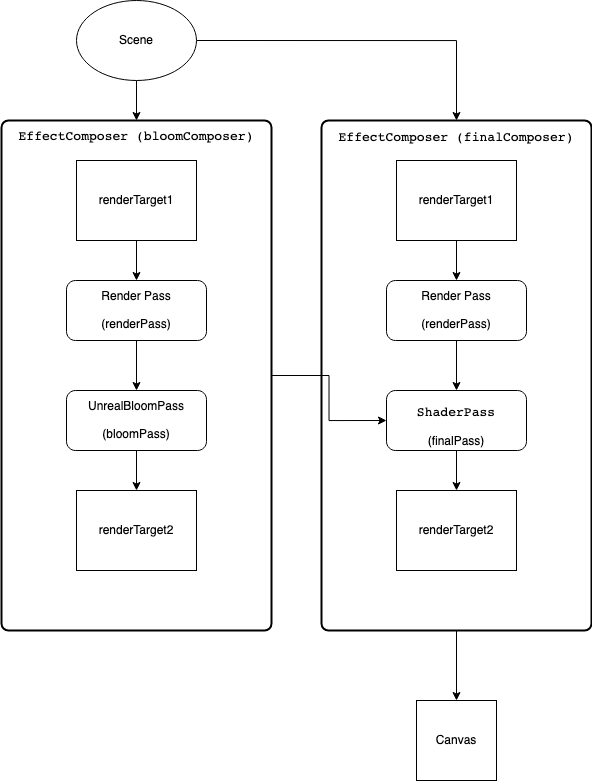
\includegraphics[width=0.5\linewidth]{../../screenshots/images/render.png}
  \caption{\label{fig:renderingPipelien} Rendering Pipeline: From 3D scene to canvas}
\end{figure}

\end{frame}


\begin{frame}
\frametitle{Implementation - Color Scheme}
% The color scheme of our approach is, that each kind of anatomical structure of the heart is colored in just one color. We used this more abstract coloring scheme proposed by the authors of the data set because this project focuses on learn- ing the different parts of the organ and their relative position to one another and less on the realism of the visualization result.
% Regarding the vessels we have to point out, that the coloring follows the oxygenation of the blood they carry and not their anatomical classification, whether they are arteries or veins, resulting in red for all arteries except the pulmonary artery, as they carry oxygenated blood, and blue all veins except the pulmonary veins, because they carry deoxygenated blood. The pulmonary artery is blue, while the pulmonary veins are red.

\begin{table}[h]
\begin{tabular}{ll}
Organ strucutres           & Color \\
\hline
Coronary arteries & red   \\
Pulmonary vein    & red   \\
Aorta             & red   \\
Coronary veins    & blue   \\
Pulmonary arteries    & blue   \\
Vena cava superior and inferior    & blue   \\
Trabecular muscle    & saddlebrown   \\
Myocard    & brown   \\
Right and left Auricle    & \#ffc0a1   \\
Heart valves    & lightblue   \\
\end{tabular}
\caption{Color scheme for the different kinds of anatomical structures}
\end{table}
\end{frame}

\section{Results} 
\frametitle{Results}

\begin{frame}
\frametitle{Implementation - Interaction}
\begin{itemize}
\item 3D Interaction
\begin{itemize}
\item Rotate
\item Translate
\item Hide anatomical structures
\end{itemize}
\item  Dropdown
\begin{itemize}
\item Highlighting
\item Language selection for info panel 
\end{itemize}

\end{itemize}
\begin{figure}[htp]

\centering
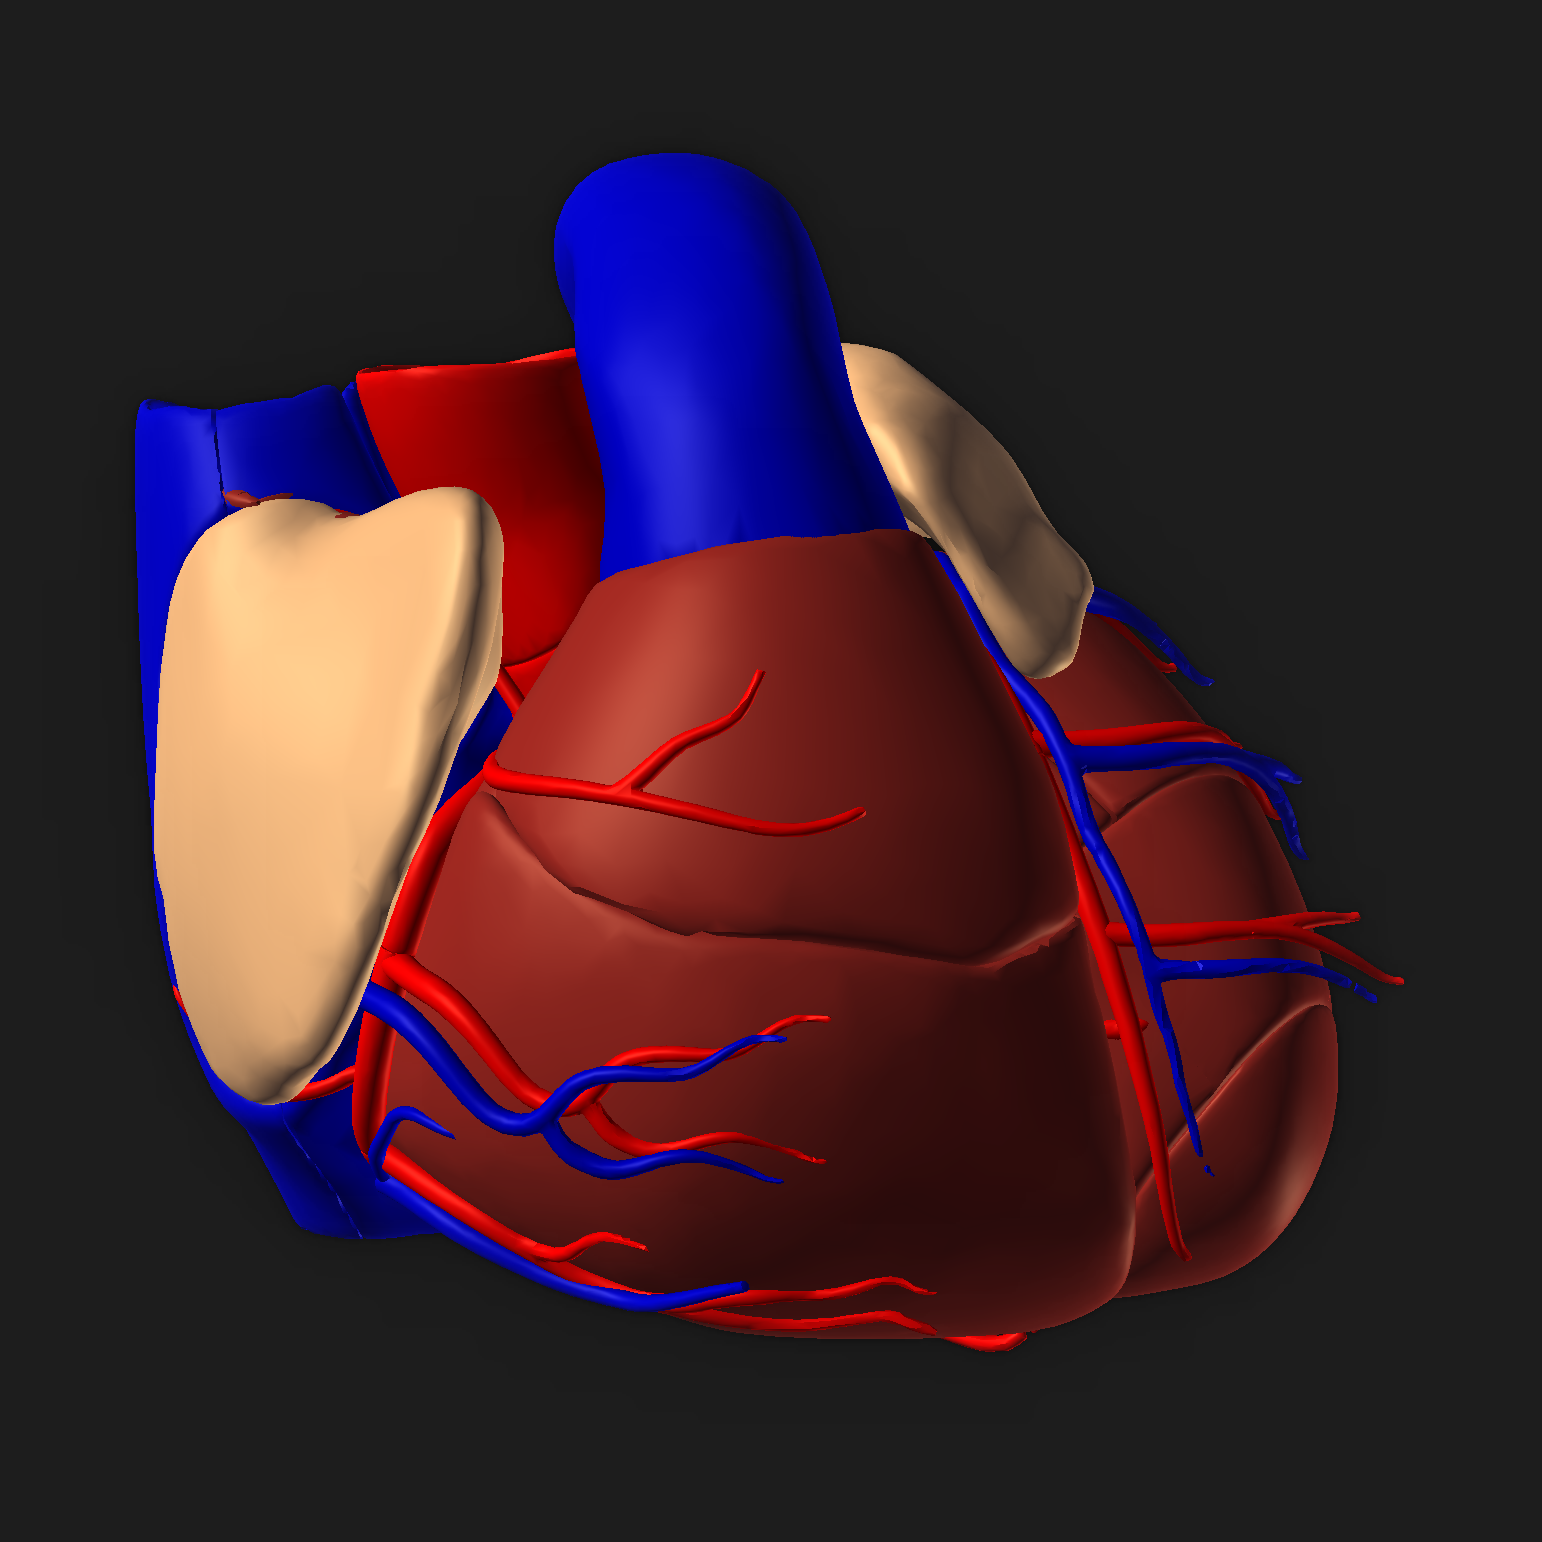
\includegraphics[width=.3\textwidth]{../../screenshots/images/example_heart.png}\hfill
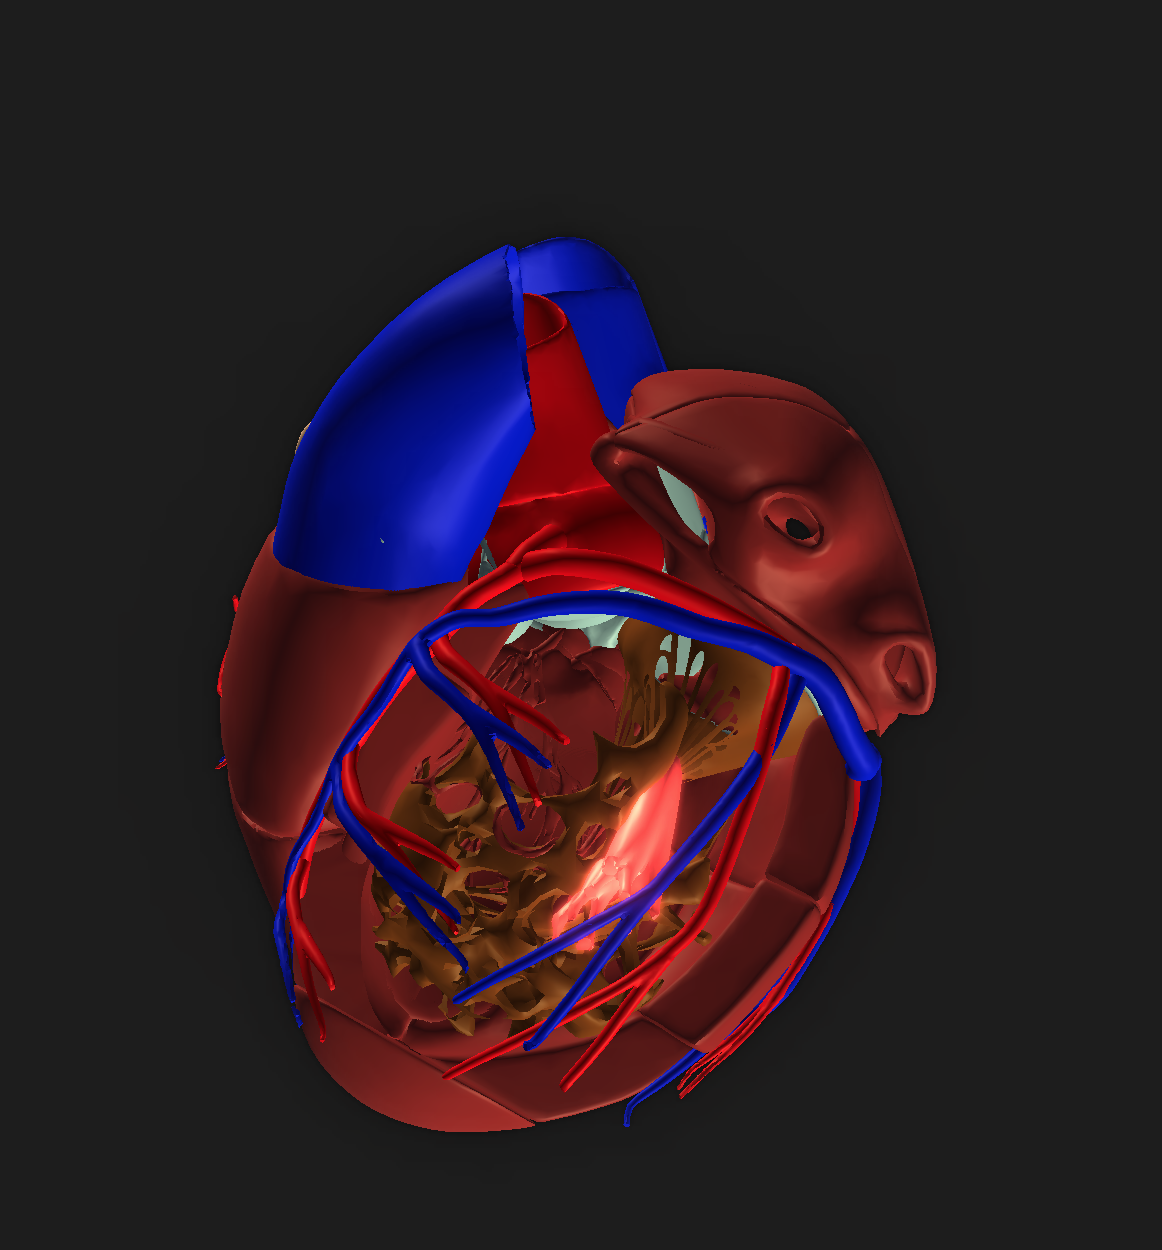
\includegraphics[width=.3\textwidth]{../../screenshots/images/LeftPapillaryMuscle_hiding.png}\hfill
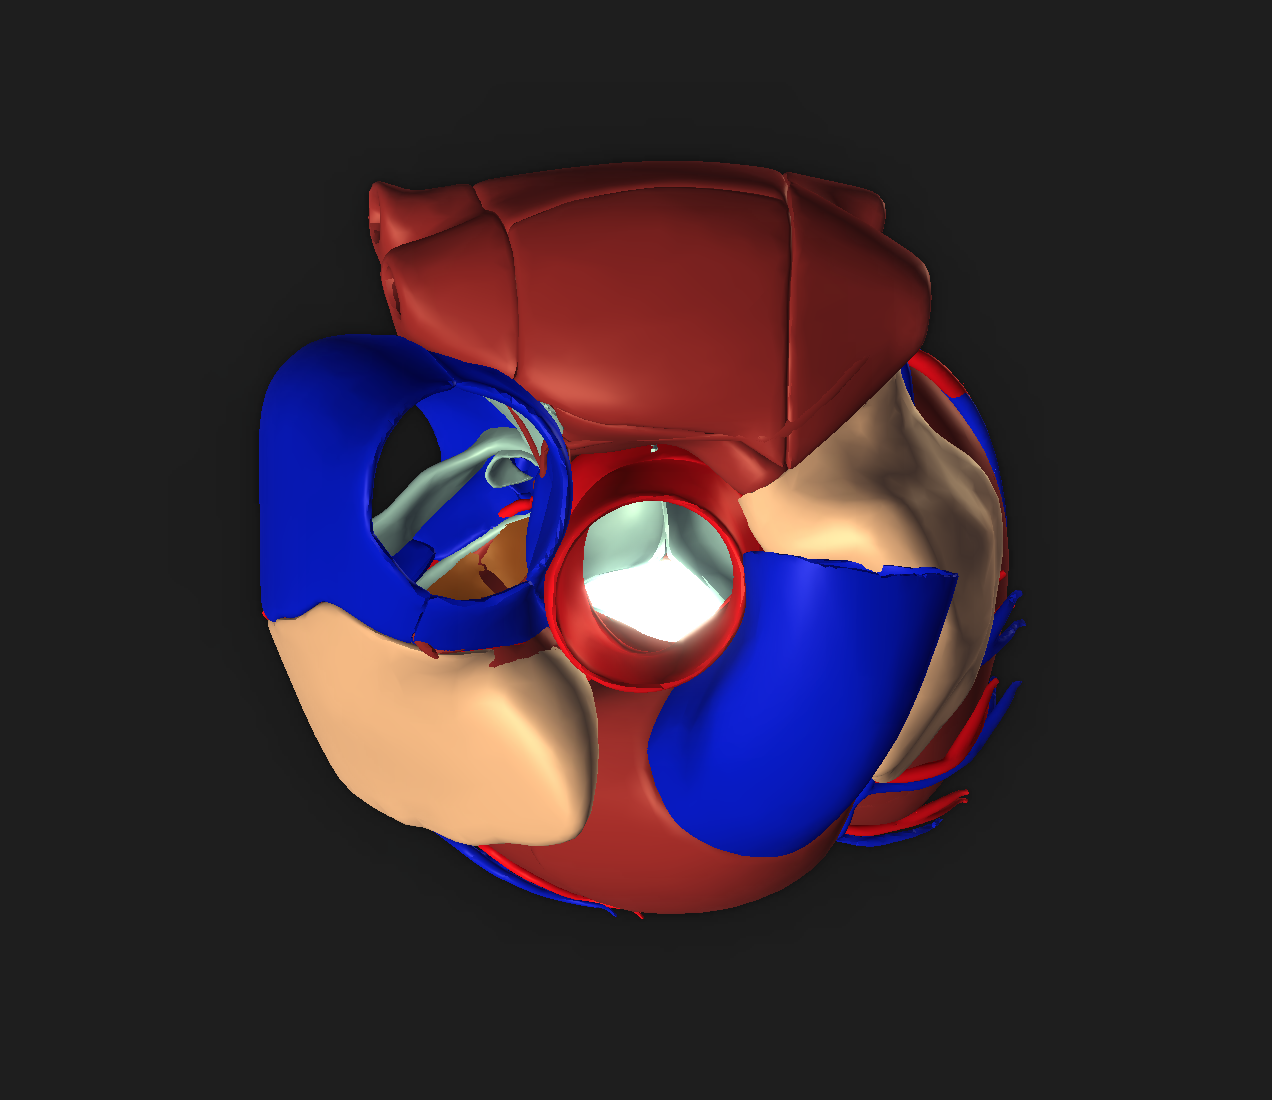
\includegraphics[width=.3\textwidth]{../../screenshots/images/aortic_valve_semilunar.png}

\end{figure}
\end{frame}


\section{Results} 
\begin{frame}
\frametitle{Results}
\begin{itemize}
\item Pure java-script interactive Three-dimensional visualization of a mesh model of the human heart for learning purposes
\item based on three.js, runs in almost any web browser
\item Supports zoom, rotation and hiding of all anatomical structures for non-occluded view of structures inside the heart
\item Selective highlighting of anatomical structures
\item Additional info panel with informations from Wikipedia in English and German
\end{itemize}
\end{frame}

\section{Discussion and outlook to future work} 
\begin{frame}
\frametitle{Discussion and outlook to future work}
\begin{itemize}
\item Develop mobile version
\item How to properly show highlighted inner structures 
\item Scientific sources instead of Wikipedia articles
\item Showing CT(A) or MR(A) imaging

% TODO could be added
%\item Feature Cross-section 
% gain better insight of the inner structures of the human heart
% TODO could be added
%\item Text field showing name of the anatomical structures
% When hovering
\end{itemize}

\begin{figure}[h]
  \centering
  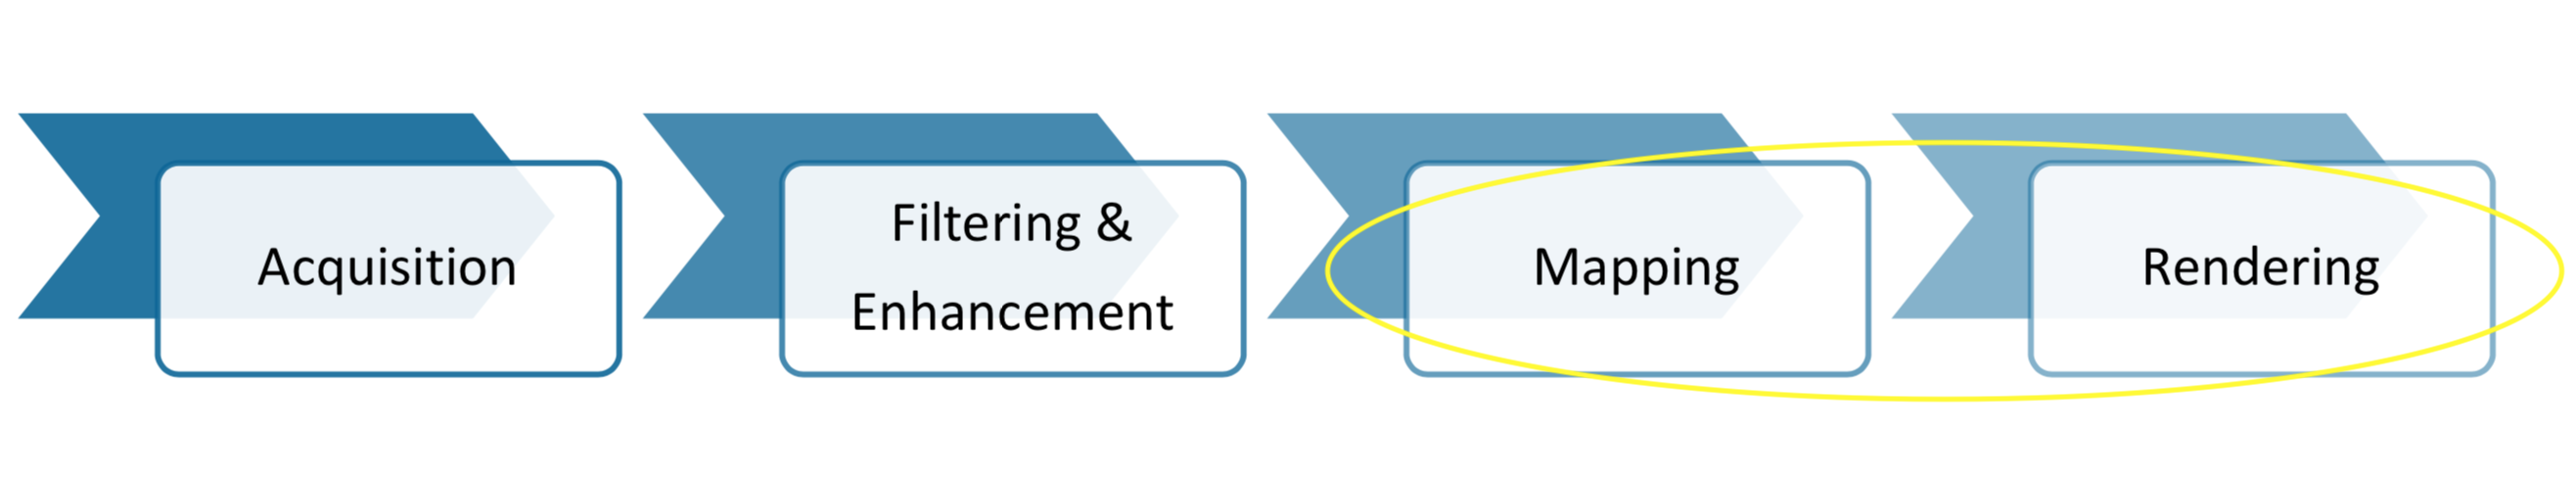
\includegraphics[width=.4\linewidth]{../../screenshots/images/renderingpipieline.png}
  \caption{Rendering pipeline of a medical visualization the slides of VisMed2, originally from \cite{p2}}
\end{figure}



\end{frame}


% BodyParts3D, © The Database Center for Life Science licensed under CC Attribution-Share Alike 2.1 Japan
\begin{frame}
\frametitle{References}
\footnotesize{
\begin{thebibliography}{99} % Beamer does not support BibTeX so references must be inserted manually as below
\bibitem[BodyParts3D, 2008]{p1} BodyParts3D (2008)
\newblock Anatomical Structure of Human Heart
\newblock \emph{The Database Center for Life Science} licensed under CC Attribution-Share Alike 2.1 Japan
\bibitem[HaberMcNabb, 1990]{p2} Haber, Robert B and McNabb, David A (1990)
\newblock Visualization idioms: A conceptual model for scientific visualization systems
\newblock \emph{Visualization in scientific computing, 74, 93}
\bibitem[Triepels et. al., 2020]{p3} Triepels, Charlotte P. R. and Smeets, Carlijn F. A. and Notten, Kim J. B. and Kruitwagen, Roy F. P. M. and Futterer, Jurgen J. and Vergeldt, Tineke F. M. and Van Kuijk, Sander M. J. (2020)
\newblock Does three-dimensional anatomy improve student understanding?
\newblock \emph{Clinical Anatomy, 33, 1, 25-33}
\bibitem[Hackett, Proctor, 2016]{p4} Hackett, M, Proctor, M.
\newblock Three-Dimensional Display Technologies for Anatomical Education: A Literature Review
\newblock \emph{Journal of Science Education and Technology, 4, 641--654}
\end{thebibliography}
}
\end{frame}


\begin{frame}
\Huge{\centerline{Thank you!}}
\end{frame}

%----------------------------------------------------------------------------------------

\end{document}